\documentclass[
	ngerman,
	points=true,% für die Aktivierung der Punktereferenzen funktioniert nicht für TeX Versionen vor 2020
    solution=true,
    accentcolor=9c,
    colorbacktitle
	]{tudaexercise}

\usepackage[english]{babel}
\usepackage[autostyle]{csquotes}
\usepackage{amsmath}
\usepackage{amssymb}
\DeclareMathOperator*{\argmin}{arg\,min}

%Formatierungen für Beispiele in diesem Dokument. Im Allgemeinen nicht notwendig!
\let\file\texttt
\let\code\texttt
\let\pck\textsf
\let\cls\textsf
\let\tbs\textbackslash

\usepackage{booktabs}% Erweiterte möglichkeiten beim Spacing um Linien in Tabellen
\renewcommand*{\creditformatsum}[1]{\creditformat{Gesamt: #1}}

\ConfigureHeadline{
	headline={title-name-id}
}

\begin{document}

\title[Homework 1/4]{Statistical Machine Learning -- Homework}
\author{Prof. Dr. Jan Peters \\ Daniel Palenicek, An Thai Le, Theo Gruner, Maximilian Tölle \& Théo Vincent}
\term{Sommersemester 2023 -- Due date: 15.05.2023, 23:59}
\sheetnumber{1}

\maketitle
Each (sub)task in this homework is worth 1 point. For example, you can get up to 3 points in task 1.1. The points you achieve in this homework will count towards the exam bonus points. \\
The solutions need to be uploaded to moodle before the deadline. You can provide us with scans of your handwritten solutions or directly write into our .tex file and submit as .pdf. Please make sure that we can exactly determine which solution belongs to which (sub)task. If you decide for handwritten solutions, please understand that we can only give points for answers which we can also read! 

\section*{Linear Algebra}
\begin{task}{Pseudo inverse}
\begin{subtask}
Can the right-pseudo inverse matrix of 
$A = 
\begin{bmatrix}
    1 & 0 & 2\\
    5 & 1 & 3
\end{bmatrix}
$ be computed? If yes, compute it. If no, explain why.
\end{subtask}
\begin{solution}

\end{solution}

\begin{subtask}
Can the left-pseudo inverse matrix of 
$B = 
\begin{bmatrix}
    1 & 7 & 2 & 3\\
    0 & 4 & 1 & 5\\
    0 & 1 & 0 & 4
\end{bmatrix}
$ be computed? If yes, compute it. If no, explain why.
\end{subtask}
\begin{solution}

\end{solution}

\begin{subtask}
Can the left-pseudo inverse matrix of 
$C = 
\begin{bmatrix}
    6 & 3 & 2\\
    0 & 2 & 4\\
    9 & 3 & 0\\
    3 & 5 & 8
\end{bmatrix}
$ be computed? If yes, compute it. If no, explain why.
\end{subtask}
\begin{solution}

\end{solution}
\end{task}

\begin{task}{Determinant}
\begin{subtask}
Compute the determinant of 
$D = 
\begin{bmatrix}
    3 & 9 & 17 & 4\\
    0 & 0 & 2  & 3\\
    0 & 0 & 5  & 1\\
    0 & 5 & 3  & 8
\end{bmatrix}
$ using Leibniz formular.
\end{subtask}
\begin{solution}

\end{solution}

\begin{subtask}
Compute the determinant of 
$E = 
\begin{bmatrix}
    0  & 4 & 7 & 0\\
    10 & 3 & 8 & 2\\
    3  & 1 & 4 & 0\\
    0  & 5 & 1 & 0
\end{bmatrix}
$ using Laplace formular.
\end{subtask}
\begin{solution}

\end{solution}

\begin{subtask}
Compute the determinant of $E^{\intercal} D^{-1}$.
\end{subtask}
\begin{solution}

\end{solution}
\end{task}

\begin{task}{Matrix decomposition}
\begin{subtask}
Compute the eigenvalues and the eigenvectors of 
$F = 
\begin{bmatrix}
    -3  & 0  & 0  \\
    -42 & 3  & -6 \\
    14  & -2 & -1
\end{bmatrix}$.\\
\textbf{Hint}: The characteristic polynomial of $F$ has a double root.
\end{subtask}
\begin{solution}

\end{solution}

\begin{subtask}
Let $G \in \mathbb{R}^{n \times n}, n \in \mathbb{N}$ be a positive definite symetric matrix. Show that there exists $H \in \mathbb{R}^{n \times n}$ such that $G = H^2$.
\end{subtask}
\begin{solution}

\end{solution}
\end{task}

\newpage

\section*{Statistics}
In this section, you are not allowed to use any kind of formula without adding its proof.
\begin{task}{Variances \& Covariances}
\textbf{Hint:} $\mathbb{E}\left[ X^2 \right] = \mathbb{E}[X (X - 1)] + \mathbb{E}[X]$.
\begin{subtask}
Compute the variance of $X$ a random variable following a geometric distribution in function of its parameter $p$.
\end{subtask}
\begin{solution}

\end{solution}

\begin{subtask}
Compute the covariance between $X$ a random variable following a poisson distribution and $Y$ a random variable following a binomial distribution in function of the parameters $\lambda, n, p$. If the question seems unsolvable at first sight, you are allowed to add one more assumption on the relationship between $X$ and $Y$.
\end{subtask}
\begin{solution}

\end{solution}

\begin{subtask}
Compute the covariance between $X$ a random variable following a poisson distribution and $Y = X^2 - 3X + 2$ in function of the parameter $\lambda$.
\end{subtask}
\begin{solution}

\end{solution}
\end{task}

\begin{task}{Exponential family}
\begin{subtask}
Is the uniform distribution part of the exponential family? Justify the answer.
\end{subtask}
\begin{solution}

\end{solution}
\end{task}

\begin{task}{Central Limit Theorem [coding question]}
\begin{subtask}
For this question, add the code to the answer. It should not be more than 30 lines of code. Using Python, show the effect of the Central Limit Theorem by reproducing the 3 plots of slide 22/47 for an exponential distribution with $\lambda = 2$. In addition, you are only allowed to sample from a uniform distribution. Explain what is happening in the 3 plots.
\end{subtask}
\begin{solution}

\end{solution}
\end{task}

\begin{task}{KL Divergence}
\begin{subtask}
Let $p$ be a PDF. We set $p(x) = \frac{1}{2} \mathcal{N}(x| \mu, \sigma^2) + \frac{1}{2} \mathcal{N}(x|\lambda, \gamma^2)$. Let $q$ be the PDF of $\mathcal{N}(\alpha, \beta^2)$. Find $\alpha^*, \beta^*$ such that $(\alpha^*, \beta^*) = \argmin_{\alpha, \beta} D_{\text{KL}}(p, q)$.  
\end{subtask}
\begin{solution}

\end{solution}

\begin{subtask}
When $\mu = 1, \lambda = 10, \sigma = 1$ and $\gamma = 1.5$, the solution of $\argmin_{\alpha, \beta} D_{\text{KL}}(q, p)$ is $(\alpha^{**}, \beta^{**}) = (10, 1.5)$. Using python, draw the obtained solution of the previous question along with the solution given in this question and the distribution $p$. Comment on the different behaviours by giving the intuition behind the minimizers.

The code is not expected for this question.
\end{subtask}
\begin{solution}

\end{solution}
\end{task}

\begin{task}{Manipulating Gaussians}
\begin{subtask}
Let $A \in \mathbb{R}^{n \times n}, n \in \mathbb{N}^*, b \in \mathbb{R}^n, X \sim \mathcal{N}(\mu, \Sigma)$ with $\mu \in \mathbb{R}^n$ and $\Sigma \in \mathbb{R}^{n \times n}$. Let $\epsilon \sim \mathcal{N}(0, \Sigma_{\epsilon})$. Which distribution is $Y = AX + b + \epsilon$ following? Compute its parameters in function of $A, b, \mu, \Sigma, \Sigma_{\epsilon}$.

\textbf{Hint:} You can use the fact without proving it that the characterictic function of $X$ is, for $t \in \mathbb{R}^n$: $\phi_X(t) = \mathbb{E}(e^{it^{\intercal}\mu - \frac{1}{2}t^{\intercal}\Sigma t})$.
\end{subtask}
\begin{solution}

\end{solution}
\end{task}

\newpage

\section*{Optimization}
\begin{task}{Convexity}
For $ n=1,...,N$ input samples $(\mathbf{x}_n, y_n)$, we want to find the weights $\mathbf{w}$ that minimize the differentiable cost function
\begin{equation*}
    \mathcal{J}(\textbf{w})= \frac{1}{2} \| \textbf{X}\textbf{w}-\mathbf{y} \|_{2}^{2}.
\end{equation*}
Proof under which conditions for \textbf{X} and \textbf{y} a unique global minimum exists. Provide the unique solution $\textbf{w}^{*}$. \\
\textbf{Hint}: Use the Hessian. 

\begin{solution}

\end{solution}
\end{task}
\begin{task}{Numerical Optimization}
Given is the following cost function 
\begin{equation*}
    \mathcal{J}(\textbf{w})=-\frac{1}{N}\sum_{n=1}^{N}[y_{n}\log\left(\sigma(\mathbf{w}^\intercal\mathbf{x}_n)\right)+(1-y_n)\log\left(1-\sigma(\mathbf{w}^\intercal\mathbf{x}_n)\right)]
\end{equation*}
with 
\begin{equation*}
    \sigma(\mathbf{w}^\intercal\mathbf{x}_n)=\frac{1}{1+e^{-\mathbf{w}^\intercal\mathbf{x}_n}}
\end{equation*}
being the sigmoid function.
\begin{subtask}
As we are not able to find a closed-form solution, we fall back to a numerical optimization method. Here, we would like to use \textbf{stochastic gradient descent} to minimize the cost function. Please derive the corresponding update rule. Then express your derived update rule in matrix form.
\end{subtask}
\begin{solution}

\end{solution}

\begin{subtask}
Does the cost function have a local or global minimum? Please proof your answer. \\
\textbf{Hint}: Use the Hessian.
\end{subtask}
\begin{solution}
    
\end{solution}
\begin{subtask}
Stochastic gradient descent is a prominent but slow optimization algorithm. Under the assumption of convergence, can Newton's method increase convergence speed? Consider the following two criteria in your answer: number of optimization steps until convergence and computing time per optimization step. 
\end{subtask}
\begin{solution}

\end{solution}
\end{task}

\begin{task}{Lagrange multiplier}
Given is the constrained optimization problem:
\begin{align*}
    & \min_{\mathbf{w}, b} \quad \frac{1}{2}\| \mathbf{w}\|^{2} \\
    & \text{s.t.} \quad y_{n}(\mathbf{w}^\intercal\mathbf{x}_n+b)\geq 1 \quad \text{for} \quad n=1, ..., N
\end{align*}
\textbf{Hint}: For the following tasks, the KKT-conditions should be considered ($\lambda_n$: Lagrange multiplier, $f_n(\mathbf{w}, b)$: constraint)
\begin{align*}
    \lambda_n & \geq 0 \quad \text{for} \quad n=1, ..., N \\
    f_n(\mathbf{w}, b) & \geq 0 \quad \text{for} \quad n=1, ..., N \\
    \lambda_n f_n(\mathbf{w}, b) & = 0 \quad \text{for} \quad n=1, ..., N.
\end{align*}
\begin{subtask}
Formulate the Lagrangian and solve for \textbf{w} and b. \\
\textbf{Hint}: $y_n \in \{-1, 1\}$, so $y_n^{2}=1$
\end{subtask}
\begin{solution}
    
\end{solution}

\begin{subtask}
Our primal formulation can sometimes be tricky to solve. Therefore, we would like to switch to the dual formulation. Please derive the dual formulation and define the corresponding optimization problem. You do not need to solve it!    
\end{subtask}
\begin{solution}

\end{solution}
\end{task}

\section*{Bayesian Decision Making}
\begin{task}{Bayes' Theorem}
Suppose you work for a tech company that produces two types of computer chips, A and B. The company has two factories, X and Y, that produce the chips. Factory X produces 55\% of the chips, while factory Y produces the remaining 45\%. The quality of the chips produced by factory X is such that 4\% of the chips produced by X are defective, while the quality of the chips produced by factory Y is such that 3\% of the chips produced by Y are defective. \\ \\
A customer purchases one of these chips from your company, but you don't know which factory produced the chip. The customer reports that the chip is defective. What is the probability that the chip was produced by factory X? Please derive your answer. 
\end{task}
\begin{solution}

\end{solution}

\begin{task}{Misclassification}
Within the figure, the three joint probabilities $p(x, \mathcal{C}_1)$, $p(x, \mathcal{C}_2)$ and $p(x, \mathcal{C}_3)$ are given. The initial decision regions are provided underneath as $\mathcal{R}_1$, $\mathcal{R}_2$ and $\mathcal{R}_3$. For instance, a data point $x$ within the range of decision region $\mathcal{R}_2$ will be classified as $\mathcal{C}_2$. \\
We are now going to minimize the probability of misclassification, $p(\text{error})$.    
\end{task}
\begin{subtask}
Within the figure, mark the regions under the probability distributions that will no longer contribute to $p(\text{error})$.
\begin{figure}[h]
  \centering
  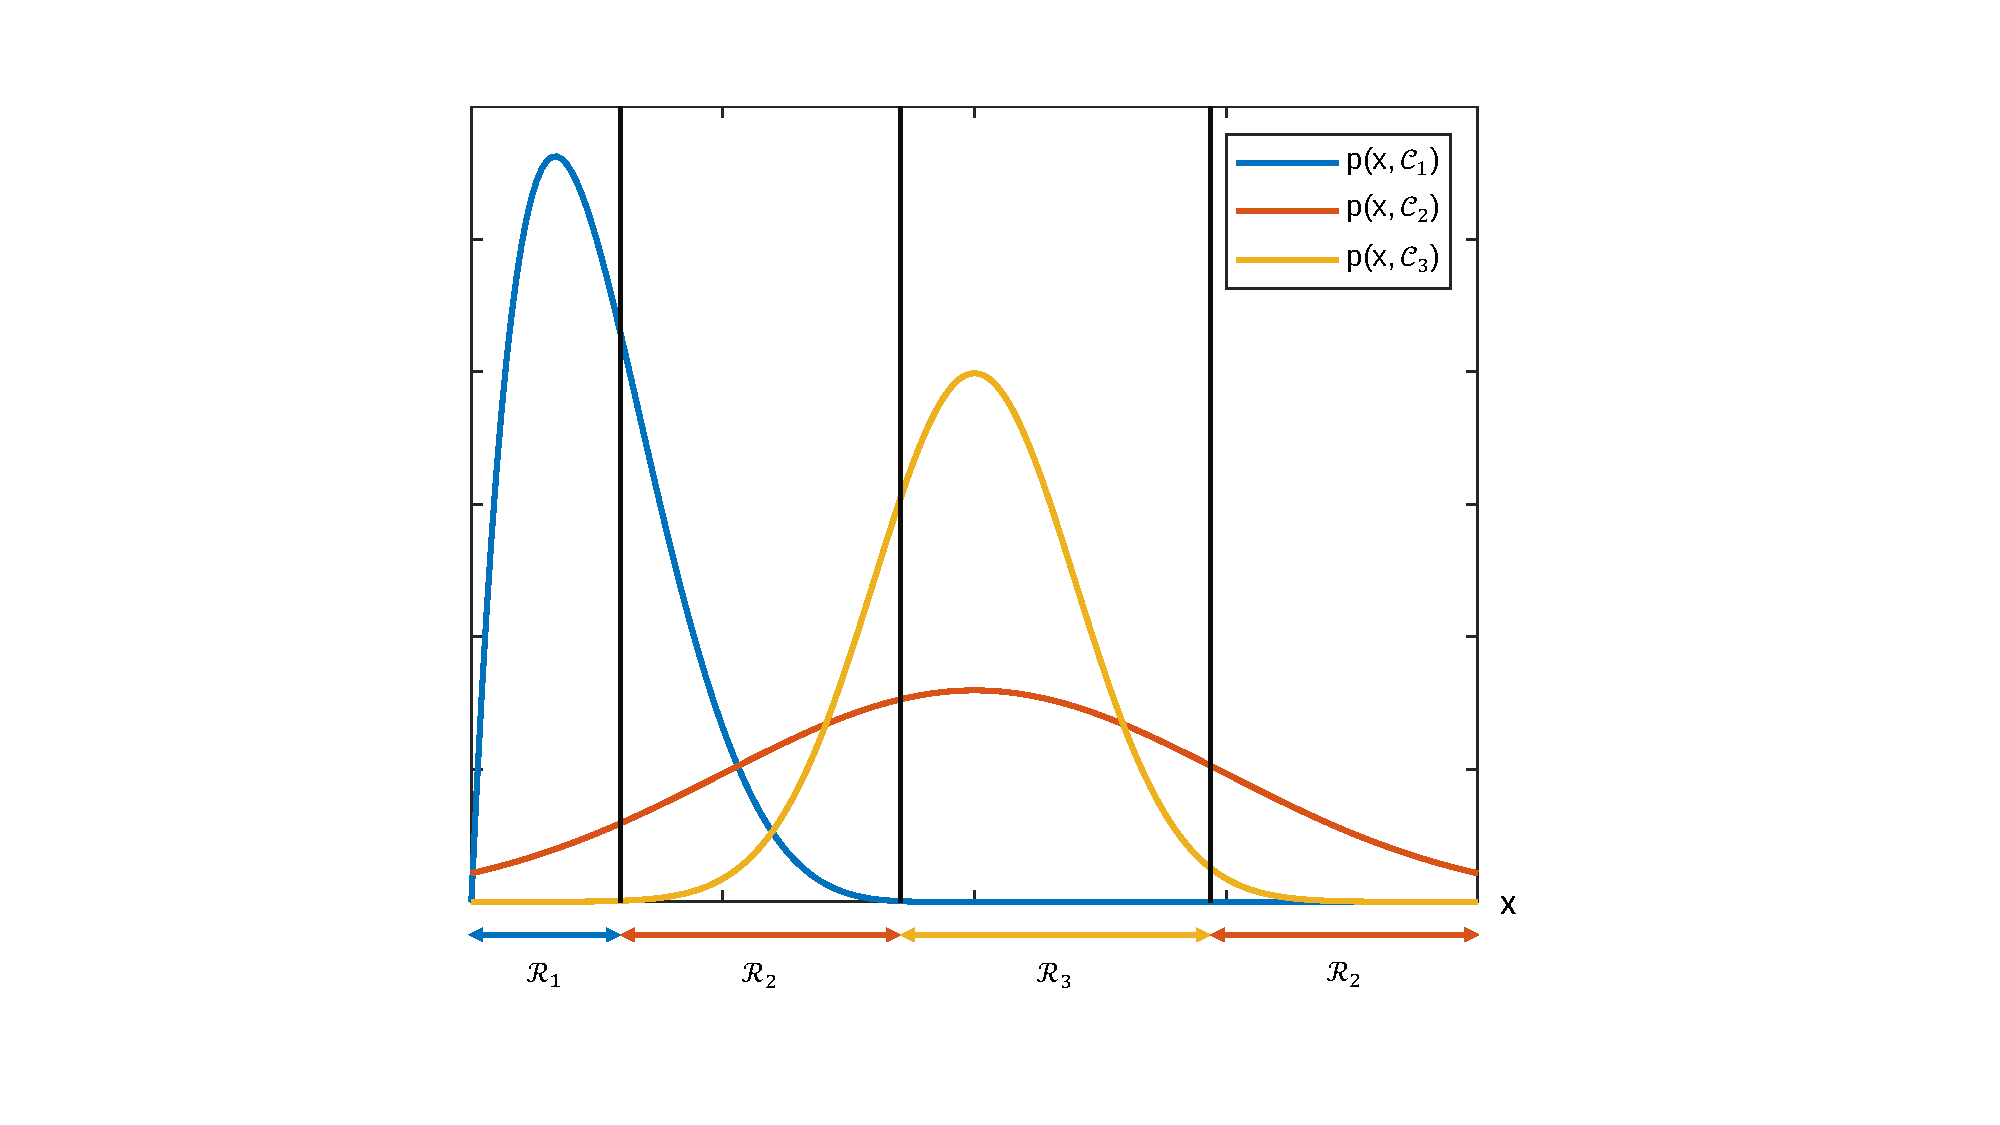
\includegraphics[width=0.6\textwidth]{misclassification.pdf}
  \label{fig:example}
\end{figure} 
\end{subtask}
\begin{subtask}
Is it possible to reduce the probability of misclassification to zero in this example? Please explain your answer.
\end{subtask}
\begin{solution}
\end{solution}

\begin{task}{Optimal Decision Boundary}
We consider discrete data of two classes $\mathcal{C}_1$ and $\mathcal{C}_2$ that is being generated by two corresponding Poisson distributions with parameters $\lambda_1$ and $\lambda_2$. For instance, class $\mathcal{C}_1$ is represented by 
\begin{equation*}
    \text{Poi}(x|\lambda_1)=e^{-\lambda_1}\frac{\lambda_1^{x}}{x!}.
\end{equation*}
Derive the optimal decision boundary $x^{*}$ analytically as a function of $\lambda_1$ and $\lambda_2$. The prior for $\mathcal{C}_1$ is given as $p(\mathcal{C}_1)=0.2$.
\end{task}
\begin{solution}
    
\end{solution}

\begin{task}{Risk Minimization}
Given is a classification problem of $N$ classes, $C=\{\mathcal{C}_1, \mathcal{C}_2, ..., \mathcal{C}_N\}$. We additionally introduce the option to assign a sample $x$ to neither of the classes which is known as $\mathcal{C}_{\text{rej}}$. When the rejection risk is lower than the risk of assignment to each class $\mathcal{C}_k\in C$, rejection can be a desirable action. Let the true class of a sample $x$ be $C_{k}$ and the class it gets assigned to during classification be $C_j$. For any $k\in\{1, 2, ..., N\}$ and $j\in\{1, 2, ..., N+1\}$, the loss is defined as 
\[
\lambda_{jk}=\begin{cases}
0  & ,\text{if} \quad j=k \\
\text{l}_{\text{reject}} & ,\text{if} \quad j=N+1 \\
\text{l}_{\text{misclassified}} & ,\text{otherwise} 
\end{cases}
\]
\begin{subtask}
Derive the decision criterion that will give the minimum expected loss. \\
\textbf{Hint}:
\[
    \text{classify}(x)\rightarrow 
    \begin{cases}
        \mathcal{C}_k  &, \text{if} \ \text{condition 1} \land \text{condition 2}\\
        \mathcal{C}_{\text{rej}} &, \text{otherwise}       
    \end{cases}
\]
\end{subtask}
\begin{solution}
    
\end{solution}

\begin{subtask}
What happens if $\text{l}_{\text{reject}}=0$?
\end{subtask}
\begin{solution}
    
\end{solution}

\begin{subtask}
What happens if $\text{l}_{\text{reject}} > \text{l}_{\text{misclassified}}$?
\end{subtask}
\begin{solution}
    
\end{solution}
\end{task}

\end{document}
